\subsubsection{Main procedure}
After the first Join-request message, the detection algorithm can no longer guarantee that a packet \(\ p \) with DevAddress \(\ a \) such that \(\ P_{a} \notin C \) necessarily belongs to a new, unregistered device. This time we have to consider also the hypothesis that the address \(\ a \) belongs to a  re-joined device. In detail, for each DevAddress \(\ a \), we have:

\vspace{3mm}
\begin{enumerate}
	\item \(\ P_{a} \in C \). \(\ a \) refers to a known ED, and it associated to a known pattern.
	\item \(\ P_{a} \notin C \). \(\ a \) refers to an unknown ED. The algorithm must recognize if it is belongs to a new device or an old one that re-joined the network.
\end{enumerate}
\vspace{3mm}

When the second scenario occurs, as in the Pre-Join procedure, a new pattern \(\ P_{a} \) is initialized. However, this time the pattern is not put in \(\ C \), but in a new vector, called \(\ U \), until the algorithm finds out if the address \(\ a \) represents a new device or not. Finally, the algorithm initialized the list \(\ TA_{a} \gets C \) of \textit{potential} patterns which could match with \(\ P_{a}\).

\vspace{5mm}

After the initialization of \(\ P_{a} \), each time the system receives as input a new packet \(\ p \) with the same address \(\ a \) and a new timestamp \(\ t \), the algorithm updates \(\ P_{a} \gets U \) and compares it with the patterns of \(\ TA_{a} \). Initially, the \(\ TA_{a} \gets verified(C) \) i.e. is it is composed of all the elements of C whose patterns is complete (then, with \textit{verified} flag set to \texttt{True}). After the updating of \(\ P_{a} \), three situations can occur:

\vspace{3mm}
\begin{enumerate}
	\item \(\ P_{a} \) doesn't match any element of \(\ TA_{a} \).
	\item The chain of \(\ P_{a} \) is a subset of one o more chains of the patterns of \(\ TA_{a} \).
	\item \(\ P_{a} \) matches \textit{exactly} with one o more elements of \(\ TA_{a} \).
\end{enumerate}
\vspace{3mm}

When the first scenario occurs, the DevAddress \(\ a \) necessarily represents a new ED. \(\ TA_{a} \) is erased from the storage and \(\ P_{a} \) is removed from \(\ U \) to be appended in \(\ C \). 

\vspace{5mm}

On the contrary, in the second case the chain of segments of \(\ P_{a} \) matches with the \textit{subchain} of one o more patterns of \(\ TA_{a} \). This implies that the chain of \(\ P_{a} \) may still be incomplete. Then the algorithm left \(\ P_{a} \) in the vector \(\ U \) and remove from \(\ TA_{a} \) all that pattern with which \(\ P_{a} \) don't match. 

\vspace{5mm}

In the last scenario, since there is a match between \(\ P_{a} \) and another pattern \(\ P_{b} \), most likely the associated addresses \(\ a \) and \(\ b \) belong to the same device. The algorithm inserts the \(\ P_{a} \) in a reservated vector, called \(\ Q \). When PIVOT will receive a new packet with DevAddress \(\ a \) such that \(\ P_{a} \in Q \), the algorithm starts the \textit{quarantine} subroutine, that will definitively confirm or reject the match between \(\ P_{a} \) and \(\ P_{b} \).

\vspace{3mm}
\begin{algorithm}
    \caption{Main procedure}
    \begin{algorithmic}[1]
        \If{$P_{a}$ n $C$}
            \State $P.update(t)$
        \Else
            \If{$P_{a}$ in $U$}
                \State $P.update(t)$
                \If{$P_{a}$ in $Q$}
                    \State quarantine procedure
                \EndIf
                \ForAll{$P_{ta}$ in $TA(a)$}
                    \If{$match(P_{a}, P_{ta})$}
                        \State $Q \gets P_{a}$
                    \Else
                        \State $TA(a).remove(P_{ta})$
                    \EndIf
                \EndFor
                \If{$TA(a)$ is empty}
                    \State new device
                    \State $C \gets P_{a}$
                \EndIf
            \Else
                \State $P \gets newPattern(a)$
                \State $U(a) \gets P$
                \State $TA(a) \gets verified(C)$
            \EndIf
        \EndIf
    \end{algorithmic}
\end{algorithm}

\newpage

\vspace{5mm}
\subsubsection{Quarantine}
\begin{figure}[t]
    \centering
    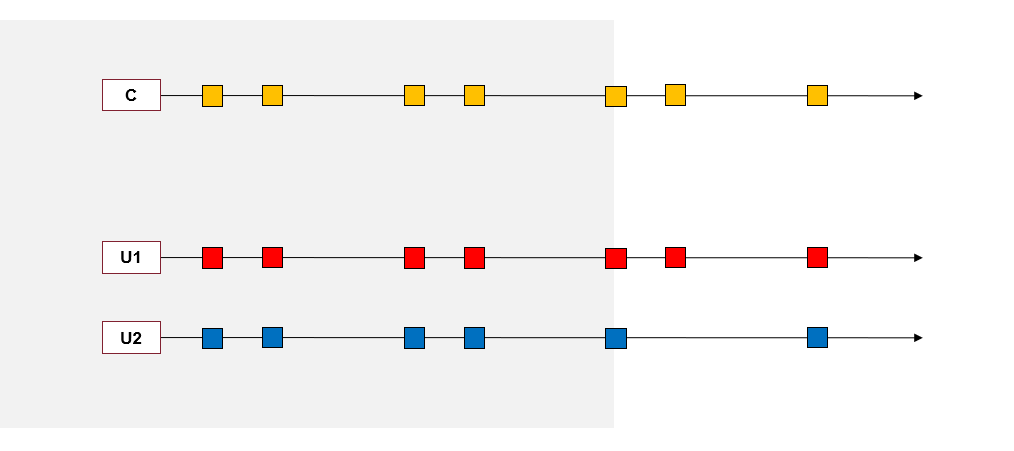
\includegraphics[width=0.7\linewidth]{images/pivot/quarantine.PNG}
    \caption{This example reports the two scenarios that can occur in the quarantine subroutine. In the first case, after updating the pattern \(\ U1 \), PIVOT confirms that \(\ U1 \) and \(\ C \) are linked to the same ED. In the second case, after updating the pattern \(\ U2 \), PIVOT confirms that \(\ U2 \) is associated to a new ED.}
    \label{fig:quarantine}
\end{figure}
When the incoming packet \(\ p \) has a DevAddress \(\ a \) such that \(\ P_{a} \in Q \), it means that \(\ P_{a} \) matches exactly with another pattern \(\ P_{b} \). The objective of the quarantine subroutine is to confirm this match or, on contrary, to demonstrate that \(\ P_{a} \) and \(\ P_{b} \) are linked to different EDs. Given the timestamp \(\ t \) of \(\ p \), the algorithm updates \(\ P_{a} \) and checks if \(\ P_{b} \) and \(\ P_{a} \) still match. If so, PIVOT triggers the \texttt{alert} the operator. If not, \(\ P_{a} \) belongs to a new device, then \(\ P_{a} \) moves from \(\ U \) to \(\ C \). The figure \ref{fig:quarantine} illustrates the two scenarios that can occur in the quarantine subroutine. Before of this step, the pattern \(\ C \) matches with both \(\ U1 \) and \(\ U2 \). In the first case, after updating \(\ U1 \) with the current timestamp \(\ t \), the algorithm confirms that \(\ U1 \) and \(\ C \) still matches. In the second case, after updating \(\ U2 \), the algorithm concluded that it represents the pattern of another device.

\vspace{3mm}
\begin{algorithm}[h!]
    \caption{Quarantine}
    \begin{algorithmic}[1]
        \State $P_{a} \gets U$
        \State $P_{b} \gets TA_{a}$
        \State $P_{a}.update(t)$
        \If{$match(P_{a}, P_{b})$}
            \State alert
        \Else
            \State new device
            \State $C \gets P_{a}$
        \EndIf
    \end{algorithmic}
\end{algorithm}
\vspace{5mm}

\newpage